\documentclass[1p]{elsarticle_modified}
%\bibliographystyle{elsarticle-num}

%\usepackage[colorlinks]{hyperref}
%\usepackage{abbrmath_seonhwa} %\Abb, \Ascr, \Acal ,\Abf, \Afrak
\usepackage{amsfonts}
\usepackage{amssymb}
\usepackage{amsmath}
\usepackage{amsthm}
\usepackage{scalefnt}
\usepackage{amsbsy}
\usepackage{kotex}
\usepackage{caption}
\usepackage{subfig}
\usepackage{color}
\usepackage{graphicx}
\usepackage{xcolor} %% white, black, red, green, blue, cyan, magenta, yellow
\usepackage{float}
\usepackage{setspace}
\usepackage{hyperref}

\usepackage{tikz}
\usetikzlibrary{arrows}

\usepackage{multirow}
\usepackage{array} % fixed length table
\usepackage{hhline}

%%%%%%%%%%%%%%%%%%%%%
\makeatletter
\renewcommand*\env@matrix[1][\arraystretch]{%
	\edef\arraystretch{#1}%
	\hskip -\arraycolsep
	\let\@ifnextchar\new@ifnextchar
	\array{*\c@MaxMatrixCols c}}
\makeatother %https://tex.stackexchange.com/questions/14071/how-can-i-increase-the-line-spacing-in-a-matrix
%%%%%%%%%%%%%%%

\usepackage[normalem]{ulem}

\newcommand{\msout}[1]{\ifmmode\text{\sout{\ensuremath{#1}}}\else\sout{#1}\fi}
%SOURCE: \msout is \stkout macro in https://tex.stackexchange.com/questions/20609/strikeout-in-math-mode

\newcommand{\cancel}[1]{
	\ifmmode
	{\color{red}\msout{#1}}
	\else
	{\color{red}\sout{#1}}
	\fi
}

\newcommand{\add}[1]{
	{\color{blue}\uwave{#1}}
}

\newcommand{\replace}[2]{
	\ifmmode
	{\color{red}\msout{#1}}{\color{blue}\uwave{#2}}
	\else
	{\color{red}\sout{#1}}{\color{blue}\uwave{#2}}
	\fi
}

\newcommand{\Sol}{\mathcal{S}} %segment
\newcommand{\D}{D} %diagram
\newcommand{\A}{\mathcal{A}} %arc


%%%%%%%%%%%%%%%%%%%%%%%%%%%%%5 test

\def\sl{\operatorname{\textup{SL}}(2,\Cbb)}
\def\psl{\operatorname{\textup{PSL}}(2,\Cbb)}
\def\quan{\mkern 1mu \triangleright \mkern 1mu}

\theoremstyle{definition}
\newtheorem{thm}{Theorem}[section]
\newtheorem{prop}[thm]{Proposition}
\newtheorem{lem}[thm]{Lemma}
\newtheorem{ques}[thm]{Question}
\newtheorem{cor}[thm]{Corollary}
\newtheorem{defn}[thm]{Definition}
\newtheorem{exam}[thm]{Example}
\newtheorem{rmk}[thm]{Remark}
\newtheorem{alg}[thm]{Algorithm}

\newcommand{\I}{\sqrt{-1}}
\begin{document}

%\begin{frontmatter}
%
%\title{Boundary parabolic representations of knots up to 8 crossings}
%
%%% Group authors per affiliation:
%\author{Yunhi Cho} 
%\address{Department of Mathematics, University of Seoul, Seoul, Korea}
%\ead{yhcho@uos.ac.kr}
%
%
%\author{Seonhwa Kim} %\fnref{s_kim}}
%\address{Center for Geometry and Physics, Institute for Basic Science, Pohang, 37673, Korea}
%\ead{ryeona17@ibs.re.kr}
%
%\author{Hyuk Kim}
%\address{Department of Mathematical Sciences, Seoul National University, Seoul 08826, Korea}
%\ead{hyukkim@snu.ac.kr}
%
%\author{Seokbeom Yoon}
%\address{Department of Mathematical Sciences, Seoul National University, Seoul, 08826,  Korea}
%\ead{sbyoon15@snu.ac.kr}
%
%\begin{abstract}
%We find all boundary parabolic representation of knots up to 8 crossings.
%
%\end{abstract}
%\begin{keyword}
%    \MSC[2010] 57M25 
%\end{keyword}
%
%\end{frontmatter}

%\linenumbers
%\tableofcontents
%
\newcommand\colored[1]{\textcolor{white}{\rule[-0.35ex]{0.8em}{1.4ex}}\kern-0.8em\color{red} #1}%
%\newcommand\colored[1]{\textcolor{white}{ #1}\kern-2.17ex	\textcolor{white}{ #1}\kern-1.81ex	\textcolor{white}{ #1}\kern-2.15ex\color{red}#1	}

{\Large $\underline{12n_{0142}~(K12n_{0142})}$}

\setlength{\tabcolsep}{10pt}
\renewcommand{\arraystretch}{1.6}
\vspace{1cm}\begin{tabular}{m{100pt}>{\centering\arraybackslash}m{274pt}}
\multirow{5}{120pt}{
	\centering
	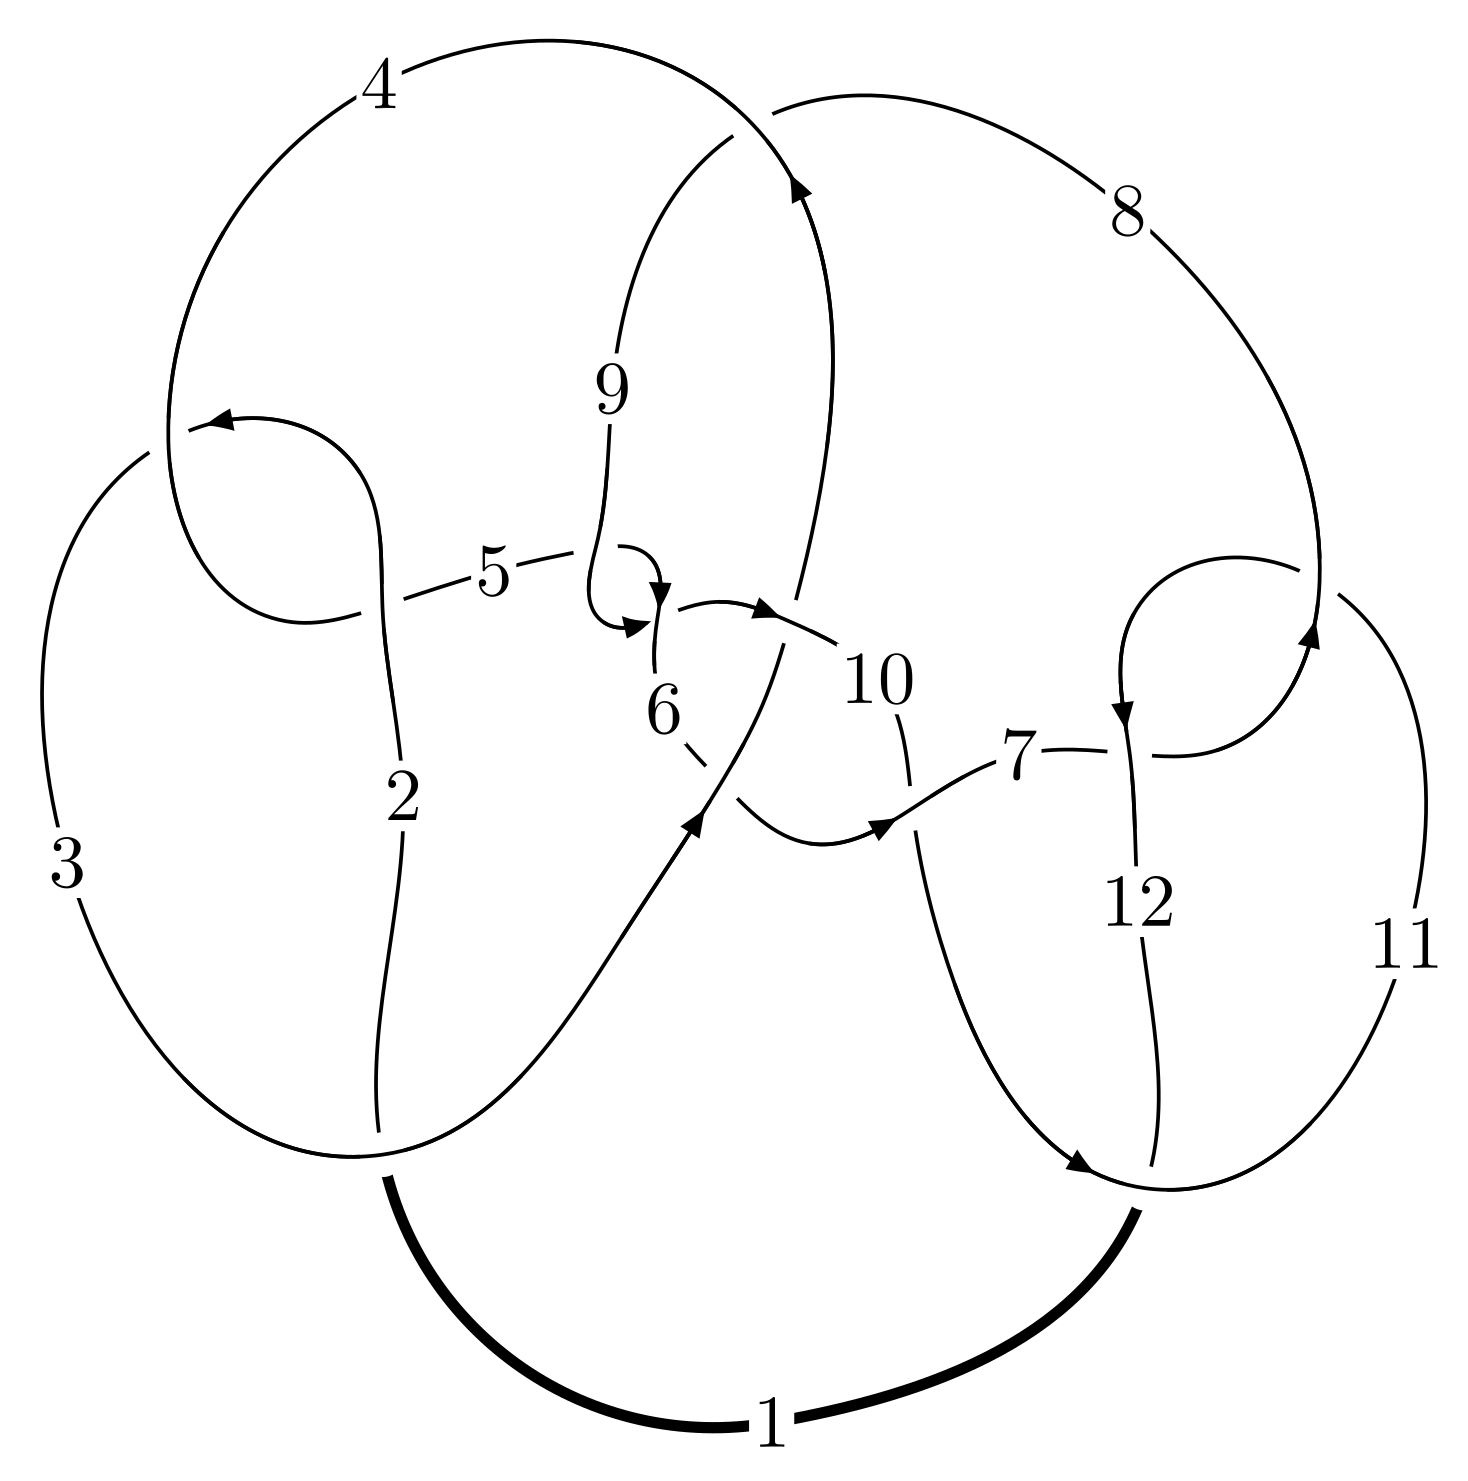
\includegraphics[width=112pt]{../../../GIT/diagram.site/Diagrams/png/2231_12n_0142.png}\\
\ \ \ A knot diagram\footnotemark}&
\allowdisplaybreaks
\textbf{Linearized knot diagam} \\
\cline{2-2}
 &
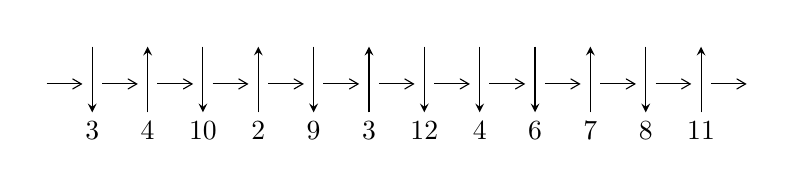
\begin{tikzpicture}[x=20pt, y=17pt]
	% nodes
	\node (C0) at (0, 0) {};
	\node (C1) at (1, 0) {};
	\node (C1U) at (1, +1) {};
	\node (C1D) at (1, -1) {3};

	\node (C2) at (2, 0) {};
	\node (C2U) at (2, +1) {};
	\node (C2D) at (2, -1) {4};

	\node (C3) at (3, 0) {};
	\node (C3U) at (3, +1) {};
	\node (C3D) at (3, -1) {10};

	\node (C4) at (4, 0) {};
	\node (C4U) at (4, +1) {};
	\node (C4D) at (4, -1) {2};

	\node (C5) at (5, 0) {};
	\node (C5U) at (5, +1) {};
	\node (C5D) at (5, -1) {9};

	\node (C6) at (6, 0) {};
	\node (C6U) at (6, +1) {};
	\node (C6D) at (6, -1) {3};

	\node (C7) at (7, 0) {};
	\node (C7U) at (7, +1) {};
	\node (C7D) at (7, -1) {12};

	\node (C8) at (8, 0) {};
	\node (C8U) at (8, +1) {};
	\node (C8D) at (8, -1) {4};

	\node (C9) at (9, 0) {};
	\node (C9U) at (9, +1) {};
	\node (C9D) at (9, -1) {6};

	\node (C10) at (10, 0) {};
	\node (C10U) at (10, +1) {};
	\node (C10D) at (10, -1) {7};

	\node (C11) at (11, 0) {};
	\node (C11U) at (11, +1) {};
	\node (C11D) at (11, -1) {8};

	\node (C12) at (12, 0) {};
	\node (C12U) at (12, +1) {};
	\node (C12D) at (12, -1) {11};
	\node (C13) at (13, 0) {};

	% arrows
	\draw[->,>={angle 60}]
	(C0) edge (C1) (C1) edge (C2) (C2) edge (C3) (C3) edge (C4) (C4) edge (C5) (C5) edge (C6) (C6) edge (C7) (C7) edge (C8) (C8) edge (C9) (C9) edge (C10) (C10) edge (C11) (C11) edge (C12) (C12) edge (C13) ;	\draw[->,>=stealth]
	(C1U) edge (C1D) (C2D) edge (C2U) (C3U) edge (C3D) (C4D) edge (C4U) (C5U) edge (C5D) (C6D) edge (C6U) (C7U) edge (C7D) (C8U) edge (C8D) (C9U) edge (C9D) (C10D) edge (C10U) (C11U) edge (C11D) (C12D) edge (C12U) ;
	\end{tikzpicture} \\
\hhline{~~} \\& 
\textbf{Solving Sequence} \\ \cline{2-2} 
 &
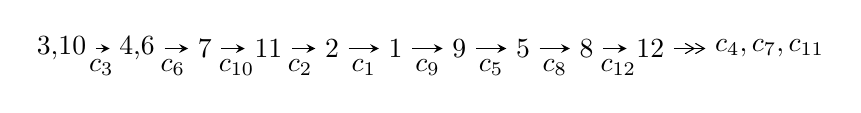
\begin{tikzpicture}[x=23pt, y=7pt]
	% node
	\node (A0) at (-1/8, 0) {3,10};
	\node (A1) at (17/16, 0) {4,6};
	\node (A2) at (17/8, 0) {7};
	\node (A3) at (25/8, 0) {11};
	\node (A4) at (33/8, 0) {2};
	\node (A5) at (41/8, 0) {1};
	\node (A6) at (49/8, 0) {9};
	\node (A7) at (57/8, 0) {5};
	\node (A8) at (65/8, 0) {8};
	\node (A9) at (73/8, 0) {12};
	\node (C1) at (1/2, -1) {$c_{3}$};
	\node (C2) at (13/8, -1) {$c_{6}$};
	\node (C3) at (21/8, -1) {$c_{10}$};
	\node (C4) at (29/8, -1) {$c_{2}$};
	\node (C5) at (37/8, -1) {$c_{1}$};
	\node (C6) at (45/8, -1) {$c_{9}$};
	\node (C7) at (53/8, -1) {$c_{5}$};
	\node (C8) at (61/8, -1) {$c_{8}$};
	\node (C9) at (69/8, -1) {$c_{12}$};
	\node (A10) at (11, 0) {$c_{4},c_{7},c_{11}$};

	% edge
	\draw[->,>=stealth]	
	(A0) edge (A1) (A1) edge (A2) (A2) edge (A3) (A3) edge (A4) (A4) edge (A5) (A5) edge (A6) (A6) edge (A7) (A7) edge (A8) (A8) edge (A9) ;
	\draw[->>,>={angle 60}]	
	(A9) edge (A10);
\end{tikzpicture} \\ 

\end{tabular} \\

\footnotetext{
The image of knot diagram is generated by the software ``\textbf{Draw programme}" developed by Andrew Bartholomew(\url{http://www.layer8.co.uk/maths/draw/index.htm\#Running-draw}), where we modified some parts for our purpose(\url{https://github.com/CATsTAILs/LinksPainter}).
}\phantom \\ \newline 
\centering \textbf{Ideals for irreducible components\footnotemark of $X_{\text{par}}$} 
 
\begin{align*}
I^u_{1}&=\langle 
2.35580\times10^{24} u^{34}+5.23556\times10^{24} u^{33}+\cdots+1.45032\times10^{25} b-1.44449\times10^{25},\\
\phantom{I^u_{1}}&\phantom{= \langle  }2.40552\times10^{24} u^{34}+8.47444\times10^{24} u^{33}+\cdots+7.25161\times10^{24} a+1.23374\times10^{25},\;u^{35}+2 u^{34}+\cdots+2 u-1\rangle \\
I^u_{2}&=\langle 
b^4+4 b^3 u-4 b^3-4 b^2 u+u-1,\;a- u+1,\;u^2- u+1\rangle \\
I^u_{3}&=\langle 
b^3-3 b^2 u-3 b^2+3 b u+1,\;a+u+1,\;u^2+u+1\rangle \\
\\
\end{align*}
\raggedright * 3 irreducible components of $\dim_{\mathbb{C}}=0$, with total 49 representations.\\
\footnotetext{All coefficients of polynomials are rational numbers. But the coefficients are sometimes approximated in decimal forms when there is not enough margin.}
\newpage
\renewcommand{\arraystretch}{1}
\centering \section*{I. $I^u_{1}= \langle 2.36\times10^{24} u^{34}+5.24\times10^{24} u^{33}+\cdots+1.45\times10^{25} b-1.44\times10^{25},\;2.41\times10^{24} u^{34}+8.47\times10^{24} u^{33}+\cdots+7.25\times10^{24} a+1.23\times10^{25},\;u^{35}+2 u^{34}+\cdots+2 u-1 \rangle$}
\flushleft \textbf{(i) Arc colorings}\\
\begin{tabular}{m{7pt} m{180pt} m{7pt} m{180pt} }
\flushright $a_{3}=$&$\begin{pmatrix}1\\0\end{pmatrix}$ \\
\flushright $a_{10}=$&$\begin{pmatrix}0\\u\end{pmatrix}$ \\
\flushright $a_{4}=$&$\begin{pmatrix}1\\u^2\end{pmatrix}$ \\
\flushright $a_{6}=$&$\begin{pmatrix}-0.331722 u^{34}-1.16863 u^{33}+\cdots-6.30773 u-1.70134\\-0.162433 u^{34}-0.360993 u^{33}+\cdots+0.130097 u+0.995980\end{pmatrix}$ \\
\flushright $a_{7}=$&$\begin{pmatrix}-0.494155 u^{34}-1.52962 u^{33}+\cdots-6.17763 u-0.705356\\-0.162433 u^{34}-0.360993 u^{33}+\cdots+0.130097 u+0.995980\end{pmatrix}$ \\
\flushright $a_{11}=$&$\begin{pmatrix}0.593442 u^{34}+0.968496 u^{33}+\cdots-3.97361 u+2.63388\\-0.474317 u^{34}-1.15537 u^{33}+\cdots+1.27477 u+0.0691574\end{pmatrix}$ \\
\flushright $a_{2}=$&$\begin{pmatrix}u^2+1\\u^4\end{pmatrix}$ \\
\flushright $a_{1}=$&$\begin{pmatrix}u^4+u^2+1\\u^4\end{pmatrix}$ \\
\flushright $a_{9}=$&$\begin{pmatrix}1.46457 u^{34}+3.18756 u^{33}+\cdots-3.14002 u+2.39592\\-0.396812 u^{34}-1.06370 u^{33}+\cdots-0.108352 u+0.168805\end{pmatrix}$ \\
\flushright $a_{5}=$&$\begin{pmatrix}u^4+u^2+1\\u^6+u^2\end{pmatrix}$ \\
\flushright $a_{8}=$&$\begin{pmatrix}1.03514 u^{34}+2.01243 u^{33}+\cdots-4.19611 u+2.30630\\-0.466022 u^{34}-1.17415 u^{33}+\cdots+0.0947758 u-0.147474\end{pmatrix}$ \\
\flushright $a_{12}=$&$\begin{pmatrix}-0.214267 u^{34}-0.843549 u^{33}+\cdots-2.91396 u+3.23369\\-0.447509 u^{34}-0.903401 u^{33}+\cdots+3.98711 u-0.173391\end{pmatrix}$\\&\end{tabular}
\flushleft \textbf{(ii) Obstruction class $= -1$}\\~\\
\flushleft \textbf{(iii) Cusp Shapes $= \frac{293178633293666810040513}{1812902632604430856362551} u^{34}-\frac{1485220871768859334081099}{7251610530417723425450204} u^{33}+\cdots-\frac{22519370902193600570526111}{1812902632604430856362551} u-\frac{6630145935705280334996315}{3625805265208861712725102}$}\\~\\
\newpage\renewcommand{\arraystretch}{1}
\flushleft \textbf{(iv) u-Polynomials at the component}\newline \\
\begin{tabular}{m{50pt}|m{274pt}}
Crossings & \hspace{64pt}u-Polynomials at each crossing \\
\hline $$\begin{aligned}c_{1}\end{aligned}$$&$\begin{aligned}
&u^{35}+54 u^{34}+\cdots+132 u-1
\end{aligned}$\\
\hline $$\begin{aligned}c_{2},c_{4}\end{aligned}$$&$\begin{aligned}
&u^{35}-6 u^{34}+\cdots-4 u+1
\end{aligned}$\\
\hline $$\begin{aligned}c_{3}\end{aligned}$$&$\begin{aligned}
&u^{35}+2 u^{34}+\cdots+2 u-1
\end{aligned}$\\
\hline $$\begin{aligned}c_{5},c_{9}\end{aligned}$$&$\begin{aligned}
&u^{35}+3 u^{34}+\cdots-83 u+13
\end{aligned}$\\
\hline $$\begin{aligned}c_{6}\end{aligned}$$&$\begin{aligned}
&u^{35}+2 u^{34}+\cdots+178664 u+28669
\end{aligned}$\\
\hline $$\begin{aligned}c_{7},c_{11}\end{aligned}$$&$\begin{aligned}
&u^{35}+u^{34}+\cdots+4 u+4
\end{aligned}$\\
\hline $$\begin{aligned}c_{8}\end{aligned}$$&$\begin{aligned}
&u^{35}-2 u^{34}+\cdots+342120 u+112661
\end{aligned}$\\
\hline $$\begin{aligned}c_{10}\end{aligned}$$&$\begin{aligned}
&u^{35}- u^{34}+\cdots-1020 u+404
\end{aligned}$\\
\hline $$\begin{aligned}c_{12}\end{aligned}$$&$\begin{aligned}
&u^{35}-15 u^{34}+\cdots-80 u+16
\end{aligned}$\\
\hline
\end{tabular}\\~\\
\newpage\renewcommand{\arraystretch}{1}
\flushleft \textbf{(v) Riley Polynomials at the component}\newline \\
\begin{tabular}{m{50pt}|m{274pt}}
Crossings & \hspace{64pt}Riley Polynomials at each crossing \\
\hline $$\begin{aligned}c_{1}\end{aligned}$$&$\begin{aligned}
&y^{35}-138 y^{34}+\cdots+4900 y-1
\end{aligned}$\\
\hline $$\begin{aligned}c_{2},c_{4}\end{aligned}$$&$\begin{aligned}
&y^{35}+54 y^{34}+\cdots+132 y-1
\end{aligned}$\\
\hline $$\begin{aligned}c_{3}\end{aligned}$$&$\begin{aligned}
&y^{35}+6 y^{34}+\cdots-4 y-1
\end{aligned}$\\
\hline $$\begin{aligned}c_{5},c_{9}\end{aligned}$$&$\begin{aligned}
&y^{35}-55 y^{34}+\cdots-1795 y-169
\end{aligned}$\\
\hline $$\begin{aligned}c_{6}\end{aligned}$$&$\begin{aligned}
&y^{35}+42 y^{34}+\cdots-5590382760 y-821911561
\end{aligned}$\\
\hline $$\begin{aligned}c_{7},c_{11}\end{aligned}$$&$\begin{aligned}
&y^{35}+15 y^{34}+\cdots-80 y-16
\end{aligned}$\\
\hline $$\begin{aligned}c_{8}\end{aligned}$$&$\begin{aligned}
&y^{35}-90 y^{34}+\cdots-117701124860 y-12692500921
\end{aligned}$\\
\hline $$\begin{aligned}c_{10}\end{aligned}$$&$\begin{aligned}
&y^{35}+15 y^{34}+\cdots-4334416 y-163216
\end{aligned}$\\
\hline $$\begin{aligned}c_{12}\end{aligned}$$&$\begin{aligned}
&y^{35}+15 y^{34}+\cdots+768 y-256
\end{aligned}$\\
\hline
\end{tabular}\\~\\
\newpage\flushleft \textbf{(vi) Complex Volumes and Cusp Shapes}
$$\begin{array}{c|c|c}  
\text{Solutions to }I^u_{1}& \I (\text{vol} + \sqrt{-1}CS) & \text{Cusp shape}\\
 \hline 
\begin{aligned}
u &= -0.604506 + 0.837594 I \\
a &= -0.448438 - 0.357846 I \\
b &= \phantom{-}0.689783 + 0.188000 I\end{aligned}
 & -0.48340 + 2.36916 I & \phantom{-}1.57611 - 4.50521 I \\ \hline\begin{aligned}
u &= -0.604506 - 0.837594 I \\
a &= -0.448438 + 0.357846 I \\
b &= \phantom{-}0.689783 - 0.188000 I\end{aligned}
 & -0.48340 - 2.36916 I & \phantom{-}1.57611 + 4.50521 I \\ \hline\begin{aligned}
u &= \phantom{-}0.390242 + 0.879154 I \\
a &= \phantom{-}0.310445 - 0.133927 I \\
b &= -0.23755 + 1.43913 I\end{aligned}
 & \phantom{-}2.56414 - 5.90559 I & \phantom{-}4.16775 + 8.40016 I \\ \hline\begin{aligned}
u &= \phantom{-}0.390242 - 0.879154 I \\
a &= \phantom{-}0.310445 + 0.133927 I \\
b &= -0.23755 - 1.43913 I\end{aligned}
 & \phantom{-}2.56414 + 5.90559 I & \phantom{-}4.16775 - 8.40016 I \\ \hline\begin{aligned}
u &= \phantom{-}0.291312 + 0.893061 I \\
a &= -0.518425 + 1.133840 I \\
b &= \phantom{-}1.01576 - 1.21326 I\end{aligned}
 & -0.669990 - 1.198850 I & \phantom{-}0.589488 - 0.204869 I \\ \hline\begin{aligned}
u &= \phantom{-}0.291312 - 0.893061 I \\
a &= -0.518425 - 1.133840 I \\
b &= \phantom{-}1.01576 + 1.21326 I\end{aligned}
 & -0.669990 + 1.198850 I & \phantom{-}0.589488 + 0.204869 I \\ \hline\begin{aligned}
u &= \phantom{-}0.201059 + 0.882276 I \\
a &= \phantom{-}0.570013 - 0.061429 I \\
b &= -1.146370 + 0.781662 I\end{aligned}
 & \phantom{-}3.35367 + 0.99605 I & \phantom{-}6.08668 + 0.22244 I \\ \hline\begin{aligned}
u &= \phantom{-}0.201059 - 0.882276 I \\
a &= \phantom{-}0.570013 + 0.061429 I \\
b &= -1.146370 - 0.781662 I\end{aligned}
 & \phantom{-}3.35367 - 0.99605 I & \phantom{-}6.08668 - 0.22244 I \\ \hline\begin{aligned}
u &= -0.396959 + 0.761909 I \\
a &= \phantom{-}0.353852 - 0.098553 I \\
b &= -0.252788 - 0.797693 I\end{aligned}
 & \phantom{-}0.24170 + 1.75473 I & -0.43635 - 4.44927 I \\ \hline\begin{aligned}
u &= -0.396959 - 0.761909 I \\
a &= \phantom{-}0.353852 + 0.098553 I \\
b &= -0.252788 + 0.797693 I\end{aligned}
 & \phantom{-}0.24170 - 1.75473 I & -0.43635 + 4.44927 I\\
 \hline 
 \end{array}$$\newpage$$\begin{array}{c|c|c}  
\text{Solutions to }I^u_{1}& \I (\text{vol} + \sqrt{-1}CS) & \text{Cusp shape}\\
 \hline 
\begin{aligned}
u &= \phantom{-}0.985569 + 0.598689 I \\
a &= -1.338090 + 0.075762 I \\
b &= \phantom{-}0.543514 - 1.234170 I\end{aligned}
 & -5.47439 - 0.97053 I & -6.95717 + 0.21297 I \\ \hline\begin{aligned}
u &= \phantom{-}0.985569 - 0.598689 I \\
a &= -1.338090 - 0.075762 I \\
b &= \phantom{-}0.543514 + 1.234170 I\end{aligned}
 & -5.47439 + 0.97053 I & -6.95717 - 0.21297 I \\ \hline\begin{aligned}
u &= -0.975167 + 0.760910 I \\
a &= -1.202040 + 0.021054 I \\
b &= \phantom{-}1.02372 + 1.38759 I\end{aligned}
 & -4.82985 + 6.52855 I & -5.30987 - 5.93880 I \\ \hline\begin{aligned}
u &= -0.975167 - 0.760910 I \\
a &= -1.202040 - 0.021054 I \\
b &= \phantom{-}1.02372 - 1.38759 I\end{aligned}
 & -4.82985 - 6.52855 I & -5.30987 + 5.93880 I \\ \hline\begin{aligned}
u &= -0.704227 + 1.101200 I \\
a &= -0.164791 - 1.088000 I \\
b &= -0.89159 + 1.41508 I\end{aligned}
 & -3.55483 - 0.18354 I & -5.27168 + 1.44891 I \\ \hline\begin{aligned}
u &= -0.704227 - 1.101200 I \\
a &= -0.164791 + 1.088000 I \\
b &= -0.89159 - 1.41508 I\end{aligned}
 & -3.55483 + 0.18354 I & -5.27168 - 1.44891 I \\ \hline\begin{aligned}
u &= \phantom{-}0.581677 + 1.185630 I \\
a &= -0.272346 + 1.132270 I \\
b &= -0.42884 - 2.03294 I\end{aligned}
 & -3.30526 - 4.99735 I & -4.49983 + 4.97284 I \\ \hline\begin{aligned}
u &= \phantom{-}0.581677 - 1.185630 I \\
a &= -0.272346 - 1.132270 I \\
b &= -0.42884 + 2.03294 I\end{aligned}
 & -3.30526 + 4.99735 I & -4.49983 - 4.97284 I \\ \hline\begin{aligned}
u &= -0.574590 + 0.262572 I \\
a &= \phantom{-}0.828257 - 0.616246 I \\
b &= \phantom{-}0.014775 - 0.612549 I\end{aligned}
 & -0.98087 + 1.09493 I & -5.80678 - 3.92220 I \\ \hline\begin{aligned}
u &= -0.574590 - 0.262572 I \\
a &= \phantom{-}0.828257 + 0.616246 I \\
b &= \phantom{-}0.014775 + 0.612549 I\end{aligned}
 & -0.98087 - 1.09493 I & -5.80678 + 3.92220 I\\
 \hline 
 \end{array}$$\newpage$$\begin{array}{c|c|c}  
\text{Solutions to }I^u_{1}& \I (\text{vol} + \sqrt{-1}CS) & \text{Cusp shape}\\
 \hline 
\begin{aligned}
u &= -0.978178 + 0.990672 I \\
a &= \phantom{-}0.991907 + 0.901079 I \\
b &= -0.57751 - 1.46799 I\end{aligned}
 & -10.30070 + 3.59687 I & -2.12620 - 2.06254 I \\ \hline\begin{aligned}
u &= -0.978178 - 0.990672 I \\
a &= \phantom{-}0.991907 - 0.901079 I \\
b &= -0.57751 + 1.46799 I\end{aligned}
 & -10.30070 - 3.59687 I & -2.12620 + 2.06254 I \\ \hline\begin{aligned}
u &= -1.12687 + 0.87702 I \\
a &= \phantom{-}1.01739 + 0.99553 I \\
b &= \phantom{-}0.581005 - 1.085740 I\end{aligned}
 & -15.7264 - 5.1315 I & -4.99224 + 2.26947 I \\ \hline\begin{aligned}
u &= -1.12687 - 0.87702 I \\
a &= \phantom{-}1.01739 - 0.99553 I \\
b &= \phantom{-}0.581005 + 1.085740 I\end{aligned}
 & -15.7264 + 5.1315 I & -4.99224 - 2.26947 I \\ \hline\begin{aligned}
u &= \phantom{-}0.553000 + 0.079189 I \\
a &= \phantom{-}1.19162 - 0.95512 I \\
b &= \phantom{-}0.541286 - 0.641792 I\end{aligned}
 & \phantom{-}0.51946 - 3.30014 I & -3.55846 + 2.28251 I \\ \hline\begin{aligned}
u &= \phantom{-}0.553000 - 0.079189 I \\
a &= \phantom{-}1.19162 + 0.95512 I \\
b &= \phantom{-}0.541286 + 0.641792 I\end{aligned}
 & \phantom{-}0.51946 + 3.30014 I & -3.55846 - 2.28251 I \\ \hline\begin{aligned}
u &= \phantom{-}1.11285 + 0.95383 I \\
a &= \phantom{-}1.03608 - 0.96278 I \\
b &= \phantom{-}0.35648 + 1.52175 I\end{aligned}
 & -17.5409 - 1.1078 I & -6.65030 + 1.84113 I \\ \hline\begin{aligned}
u &= \phantom{-}1.11285 - 0.95383 I \\
a &= \phantom{-}1.03608 + 0.96278 I \\
b &= \phantom{-}0.35648 - 1.52175 I\end{aligned}
 & -17.5409 + 1.1078 I & -6.65030 - 1.84113 I \\ \hline\begin{aligned}
u &= -0.93478 + 1.13030 I \\
a &= \phantom{-}1.030020 + 0.817450 I \\
b &= -1.15562 - 2.30328 I\end{aligned}
 & -14.8325 + 12.6268 I & -3.98580 - 6.37716 I \\ \hline\begin{aligned}
u &= -0.93478 - 1.13030 I \\
a &= \phantom{-}1.030020 - 0.817450 I \\
b &= -1.15562 + 2.30328 I\end{aligned}
 & -14.8325 - 12.6268 I & -3.98580 + 6.37716 I\\
 \hline 
 \end{array}$$\newpage$$\begin{array}{c|c|c}  
\text{Solutions to }I^u_{1}& \I (\text{vol} + \sqrt{-1}CS) & \text{Cusp shape}\\
 \hline 
\begin{aligned}
u &= \phantom{-}0.98846 + 1.10575 I \\
a &= \phantom{-}1.042800 - 0.852917 I \\
b &= -0.75564 + 2.24982 I\end{aligned}
 & -16.9917 - 6.5550 I & -6.22803 + 2.34101 I \\ \hline\begin{aligned}
u &= \phantom{-}0.98846 - 1.10575 I \\
a &= \phantom{-}1.042800 + 0.852917 I \\
b &= -0.75564 - 2.24982 I\end{aligned}
 & -16.9917 + 6.5550 I & -6.22803 - 2.34101 I \\ \hline\begin{aligned}
u &= -0.002637 + 0.401944 I \\
a &= -0.40921 - 2.57831 I \\
b &= \phantom{-}1.287540 + 0.119160 I\end{aligned}
 & \phantom{-}0.99468 + 3.59879 I & -0.61353 - 4.53406 I \\ \hline\begin{aligned}
u &= -0.002637 - 0.401944 I \\
a &= -0.40921 + 2.57831 I \\
b &= \phantom{-}1.287540 - 0.119160 I\end{aligned}
 & \phantom{-}0.99468 - 3.59879 I & -0.61353 + 4.53406 I \\ \hline\begin{aligned}
u &= \phantom{-}0.387505\phantom{ +0.000000I} \\
a &= -3.03811\phantom{ +0.000000I} \\
b &= \phantom{-}0.784090\phantom{ +0.000000I}\end{aligned}
 & -1.97384\phantom{ +0.000000I} & -5.96760\phantom{ +0.000000I}\\
 \hline 
 \end{array}$$\newpage\newpage\renewcommand{\arraystretch}{1}
\centering \section*{II. $I^u_{2}= \langle b^4+4 b^3 u-4 b^3-4 b^2 u+u-1,\;a- u+1,\;u^2- u+1 \rangle$}
\flushleft \textbf{(i) Arc colorings}\\
\begin{tabular}{m{7pt} m{180pt} m{7pt} m{180pt} }
\flushright $a_{3}=$&$\begin{pmatrix}1\\0\end{pmatrix}$ \\
\flushright $a_{10}=$&$\begin{pmatrix}0\\u\end{pmatrix}$ \\
\flushright $a_{4}=$&$\begin{pmatrix}1\\u-1\end{pmatrix}$ \\
\flushright $a_{6}=$&$\begin{pmatrix}u-1\\b\end{pmatrix}$ \\
\flushright $a_{7}=$&$\begin{pmatrix}b+u-1\\b\end{pmatrix}$ \\
\flushright $a_{11}=$&$\begin{pmatrix}b^2 u-2 b- u+1\\b^2 u- b+u\end{pmatrix}$ \\
\flushright $a_{2}=$&$\begin{pmatrix}u\\- u\end{pmatrix}$ \\
\flushright $a_{1}=$&$\begin{pmatrix}0\\- u\end{pmatrix}$ \\
\flushright $a_{9}=$&$\begin{pmatrix}- u+1\\- b+u\end{pmatrix}$ \\
\flushright $a_{5}=$&$\begin{pmatrix}0\\u\end{pmatrix}$ \\
\flushright $a_{8}=$&$\begin{pmatrix}- b- u+1\\- b u+u\end{pmatrix}$ \\
\flushright $a_{12}=$&$\begin{pmatrix}2 b^2 u-4 b\\b^3 u- b^3- b^2 u- b^2-2 b u+b+u-1\end{pmatrix}$\\&\end{tabular}
\flushleft \textbf{(ii) Obstruction class $= 1$}\\~\\
\flushleft \textbf{(iii) Cusp Shapes $= -4 b^2 u+4 b^2+8 b u+4 u-4$}\\~\\
\newpage\renewcommand{\arraystretch}{1}
\flushleft \textbf{(iv) u-Polynomials at the component}\newline \\
\begin{tabular}{m{50pt}|m{274pt}}
Crossings & \hspace{64pt}u-Polynomials at each crossing \\
\hline $$\begin{aligned}c_{1},c_{3},c_{4}\end{aligned}$$&$\begin{aligned}
&(u^2- u+1)^4
\end{aligned}$\\
\hline $$\begin{aligned}c_{2}\end{aligned}$$&$\begin{aligned}
&(u^2+u+1)^4
\end{aligned}$\\
\hline $$\begin{aligned}c_{5}\end{aligned}$$&$\begin{aligned}
&(u+1)^8
\end{aligned}$\\
\hline $$\begin{aligned}c_{6}\end{aligned}$$&$\begin{aligned}
&u^8+4 u^7+12 u^6+16 u^5+15 u^4-8 u^3-4 u^2+1
\end{aligned}$\\
\hline $$\begin{aligned}c_{7},c_{11}\end{aligned}$$&$\begin{aligned}
&(u^4+2 u^2+2)^2
\end{aligned}$\\
\hline $$\begin{aligned}c_{8}\end{aligned}$$&$\begin{aligned}
&u^8-4 u^7+12 u^6-16 u^5+15 u^4+8 u^3-4 u^2+1
\end{aligned}$\\
\hline $$\begin{aligned}c_{9}\end{aligned}$$&$\begin{aligned}
&(u-1)^8
\end{aligned}$\\
\hline $$\begin{aligned}c_{10}\end{aligned}$$&$\begin{aligned}
&(u^4-2 u^2+2)^2
\end{aligned}$\\
\hline $$\begin{aligned}c_{12}\end{aligned}$$&$\begin{aligned}
&(u^2-2 u+2)^4
\end{aligned}$\\
\hline
\end{tabular}\\~\\
\newpage\renewcommand{\arraystretch}{1}
\flushleft \textbf{(v) Riley Polynomials at the component}\newline \\
\begin{tabular}{m{50pt}|m{274pt}}
Crossings & \hspace{64pt}Riley Polynomials at each crossing \\
\hline $$\begin{aligned}c_{1},c_{2},c_{3}\\c_{4}\end{aligned}$$&$\begin{aligned}
&(y^2+y+1)^4
\end{aligned}$\\
\hline $$\begin{aligned}c_{5},c_{9}\end{aligned}$$&$\begin{aligned}
&(y-1)^8
\end{aligned}$\\
\hline $$\begin{aligned}c_{6},c_{8}\end{aligned}$$&$\begin{aligned}
&y^8+8 y^7+46 y^6+160 y^5+387 y^4-160 y^3+46 y^2-8 y+1
\end{aligned}$\\
\hline $$\begin{aligned}c_{7},c_{11}\end{aligned}$$&$\begin{aligned}
&(y^2+2 y+2)^4
\end{aligned}$\\
\hline $$\begin{aligned}c_{10}\end{aligned}$$&$\begin{aligned}
&(y^2-2 y+2)^4
\end{aligned}$\\
\hline $$\begin{aligned}c_{12}\end{aligned}$$&$\begin{aligned}
&(y^2+4)^4
\end{aligned}$\\
\hline
\end{tabular}\\~\\
\newpage\flushleft \textbf{(vi) Complex Volumes and Cusp Shapes}
$$\begin{array}{c|c|c}  
\text{Solutions to }I^u_{2}& \I (\text{vol} + \sqrt{-1}CS) & \text{Cusp shape}\\
 \hline 
\begin{aligned}
u &= \phantom{-}0.500000 + 0.866025 I \\
a &= -0.500000 + 0.866025 I \\
b &= \phantom{-}0.344777 + 0.313008 I\end{aligned}
 & \phantom{-}0.82247 - 5.69375 I & -2.00000 + 7.46410 I \\ \hline\begin{aligned}
u &= \phantom{-}0.500000 + 0.866025 I \\
a &= -0.500000 + 0.866025 I \\
b &= -0.443461 - 0.142082 I\end{aligned}
 & \phantom{-}0.82247 + 1.63398 I & -2.00000 - 0.53590 I \\ \hline\begin{aligned}
u &= \phantom{-}0.500000 + 0.866025 I \\
a &= -0.500000 + 0.866025 I \\
b &= \phantom{-}1.44346 - 1.58997 I\end{aligned}
 & \phantom{-}0.82247 + 1.63398 I & -2.00000 - 0.53590 I \\ \hline\begin{aligned}
u &= \phantom{-}0.500000 + 0.866025 I \\
a &= -0.500000 + 0.866025 I \\
b &= \phantom{-}0.65522 - 2.04506 I\end{aligned}
 & \phantom{-}0.82247 - 5.69375 I & -2.00000 + 7.46410 I \\ \hline\begin{aligned}
u &= \phantom{-}0.500000 - 0.866025 I \\
a &= -0.500000 - 0.866025 I \\
b &= -0.443461 + 0.142082 I\end{aligned}
 & \phantom{-}0.82247 + 5.69375 I & -2.00000 - 7.46410 I \\ \hline\begin{aligned}
u &= \phantom{-}0.500000 - 0.866025 I \\
a &= -0.500000 - 0.866025 I \\
b &= \phantom{-}0.344777 - 0.313008 I\end{aligned}
 & \phantom{-}0.82247 - 1.63398 I & -2.00000 + 0.53590 I \\ \hline\begin{aligned}
u &= \phantom{-}0.500000 - 0.866025 I \\
a &= -0.500000 - 0.866025 I \\
b &= \phantom{-}1.44346 + 1.58997 I\end{aligned}
 & \phantom{-}0.82247 - 1.63398 I & -2.00000 + 0.53590 I \\ \hline\begin{aligned}
u &= \phantom{-}0.500000 - 0.866025 I \\
a &= -0.500000 - 0.866025 I \\
b &= \phantom{-}0.65522 + 2.04506 I\end{aligned}
 & \phantom{-}0.82247 + 5.69375 I & -2.00000 - 7.46410 I\\
 \hline 
 \end{array}$$\newpage\newpage\renewcommand{\arraystretch}{1}
\centering \section*{III. $I^u_{3}= \langle b^3-3 b^2 u-3 b^2+3 b u+1,\;a+u+1,\;u^2+u+1 \rangle$}
\flushleft \textbf{(i) Arc colorings}\\
\begin{tabular}{m{7pt} m{180pt} m{7pt} m{180pt} }
\flushright $a_{3}=$&$\begin{pmatrix}1\\0\end{pmatrix}$ \\
\flushright $a_{10}=$&$\begin{pmatrix}0\\u\end{pmatrix}$ \\
\flushright $a_{4}=$&$\begin{pmatrix}1\\- u-1\end{pmatrix}$ \\
\flushright $a_{6}=$&$\begin{pmatrix}- u-1\\b\end{pmatrix}$ \\
\flushright $a_{7}=$&$\begin{pmatrix}b- u-1\\b\end{pmatrix}$ \\
\flushright $a_{11}=$&$\begin{pmatrix}b^2 u+2 b- u-1\\b^2 u+b+u\end{pmatrix}$ \\
\flushright $a_{2}=$&$\begin{pmatrix}- u\\u\end{pmatrix}$ \\
\flushright $a_{1}=$&$\begin{pmatrix}0\\u\end{pmatrix}$ \\
\flushright $a_{9}=$&$\begin{pmatrix}- u-1\\b+u\end{pmatrix}$ \\
\flushright $a_{5}=$&$\begin{pmatrix}0\\- u\end{pmatrix}$ \\
\flushright $a_{8}=$&$\begin{pmatrix}b- u-1\\- b u+u\end{pmatrix}$ \\
\flushright $a_{12}=$&$\begin{pmatrix}0\\- b^2+2 b u+2 b\end{pmatrix}$\\&\end{tabular}
\flushleft \textbf{(ii) Obstruction class $= 1$}\\~\\
\flushleft \textbf{(iii) Cusp Shapes $= -2 b^2 u-2 b^2+4 b u-4 u-6$}\\~\\
\newpage\renewcommand{\arraystretch}{1}
\flushleft \textbf{(iv) u-Polynomials at the component}\newline \\
\begin{tabular}{m{50pt}|m{274pt}}
Crossings & \hspace{64pt}u-Polynomials at each crossing \\
\hline $$\begin{aligned}c_{1},c_{4}\end{aligned}$$&$\begin{aligned}
&(u^2- u+1)^3
\end{aligned}$\\
\hline $$\begin{aligned}c_{2},c_{3},c_{6}\\c_{8}\end{aligned}$$&$\begin{aligned}
&(u^2+u+1)^3
\end{aligned}$\\
\hline $$\begin{aligned}c_{5}\end{aligned}$$&$\begin{aligned}
&(u-1)^6
\end{aligned}$\\
\hline $$\begin{aligned}c_{7},c_{10},c_{11}\\c_{12}\end{aligned}$$&$\begin{aligned}
&u^6
\end{aligned}$\\
\hline $$\begin{aligned}c_{9}\end{aligned}$$&$\begin{aligned}
&(u+1)^6
\end{aligned}$\\
\hline
\end{tabular}\\~\\
\newpage\renewcommand{\arraystretch}{1}
\flushleft \textbf{(v) Riley Polynomials at the component}\newline \\
\begin{tabular}{m{50pt}|m{274pt}}
Crossings & \hspace{64pt}Riley Polynomials at each crossing \\
\hline $$\begin{aligned}c_{1},c_{2},c_{3}\\c_{4},c_{6},c_{8}\end{aligned}$$&$\begin{aligned}
&(y^2+y+1)^3
\end{aligned}$\\
\hline $$\begin{aligned}c_{5},c_{9}\end{aligned}$$&$\begin{aligned}
&(y-1)^6
\end{aligned}$\\
\hline $$\begin{aligned}c_{7},c_{10},c_{11}\\c_{12}\end{aligned}$$&$\begin{aligned}
&y^6
\end{aligned}$\\
\hline
\end{tabular}\\~\\
\newpage\flushleft \textbf{(vi) Complex Volumes and Cusp Shapes}
$$\begin{array}{c|c|c}  
\text{Solutions to }I^u_{3}& \I (\text{vol} + \sqrt{-1}CS) & \text{Cusp shape}\\
 \hline 
\begin{aligned}
u &= -0.500000 + 0.866025 I \\
a &= -0.500000 - 0.866025 I \\
b &= \phantom{-}0.500000 + 0.866025 I\end{aligned}
 & -1.64493 + 2.02988 I & -6.00000 - 3.46410 I \\ \hline\begin{aligned}
u &= -0.500000 + 0.866025 I \\
a &= -0.500000 - 0.866025 I \\
b &= \phantom{-}0.500000 + 0.866025 I\end{aligned}
 & -1.64493 + 2.02988 I & -6.00000 - 3.46410 I \\ \hline\begin{aligned}
u &= -0.500000 + 0.866025 I \\
a &= -0.500000 - 0.866025 I \\
b &= \phantom{-}0.500000 + 0.866025 I\end{aligned}
 & -1.64493 + 2.02988 I & -6.00000 - 3.46410 I \\ \hline\begin{aligned}
u &= -0.500000 - 0.866025 I \\
a &= -0.500000 + 0.866025 I \\
b &= \phantom{-}0.500000 - 0.866025 I\end{aligned}
 & -1.64493 - 2.02988 I & -6.00000 + 3.46410 I \\ \hline\begin{aligned}
u &= -0.500000 - 0.866025 I \\
a &= -0.500000 + 0.866025 I \\
b &= \phantom{-}0.500000 - 0.866025 I\end{aligned}
 & -1.64493 - 2.02988 I & -6.00000 + 3.46410 I \\ \hline\begin{aligned}
u &= -0.500000 - 0.866025 I \\
a &= -0.500000 + 0.866025 I \\
b &= \phantom{-}0.500000 - 0.866025 I\end{aligned}
 & -1.64493 - 2.02988 I & -6.00000 + 3.46410 I\\
 \hline 
 \end{array}$$\newpage
\newpage\renewcommand{\arraystretch}{1}
\centering \section*{ IV. u-Polynomials}
\begin{tabular}{m{50pt}|m{274pt}}
Crossings & \hspace{64pt}u-Polynomials at each crossing \\
\hline $$\begin{aligned}c_{1}\end{aligned}$$&$\begin{aligned}
&((u^2- u+1)^7)(u^{35}+54 u^{34}+\cdots+132 u-1)
\end{aligned}$\\
\hline $$\begin{aligned}c_{2}\end{aligned}$$&$\begin{aligned}
&((u^2+u+1)^7)(u^{35}-6 u^{34}+\cdots-4 u+1)
\end{aligned}$\\
\hline $$\begin{aligned}c_{3}\end{aligned}$$&$\begin{aligned}
&((u^2- u+1)^4)(u^2+u+1)^3(u^{35}+2 u^{34}+\cdots+2 u-1)
\end{aligned}$\\
\hline $$\begin{aligned}c_{4}\end{aligned}$$&$\begin{aligned}
&((u^2- u+1)^7)(u^{35}-6 u^{34}+\cdots-4 u+1)
\end{aligned}$\\
\hline $$\begin{aligned}c_{5}\end{aligned}$$&$\begin{aligned}
&((u-1)^6)(u+1)^8(u^{35}+3 u^{34}+\cdots-83 u+13)
\end{aligned}$\\
\hline $$\begin{aligned}c_{6}\end{aligned}$$&$\begin{aligned}
&(u^2+u+1)^3(u^8+4 u^7+12 u^6+16 u^5+15 u^4-8 u^3-4 u^2+1)\\
&\cdot(u^{35}+2 u^{34}+\cdots+178664 u+28669)
\end{aligned}$\\
\hline $$\begin{aligned}c_{7},c_{11}\end{aligned}$$&$\begin{aligned}
&u^6(u^4+2 u^2+2)^2(u^{35}+u^{34}+\cdots+4 u+4)
\end{aligned}$\\
\hline $$\begin{aligned}c_{8}\end{aligned}$$&$\begin{aligned}
&(u^2+u+1)^3(u^8-4 u^7+12 u^6-16 u^5+15 u^4+8 u^3-4 u^2+1)\\
&\cdot(u^{35}-2 u^{34}+\cdots+342120 u+112661)
\end{aligned}$\\
\hline $$\begin{aligned}c_{9}\end{aligned}$$&$\begin{aligned}
&((u-1)^8)(u+1)^6(u^{35}+3 u^{34}+\cdots-83 u+13)
\end{aligned}$\\
\hline $$\begin{aligned}c_{10}\end{aligned}$$&$\begin{aligned}
&u^6(u^4-2 u^2+2)^2(u^{35}-u^{34}+\cdots-1020 u+404)
\end{aligned}$\\
\hline $$\begin{aligned}c_{12}\end{aligned}$$&$\begin{aligned}
&u^6(u^2-2 u+2)^4(u^{35}-15 u^{34}+\cdots-80 u+16)
\end{aligned}$\\
\hline
\end{tabular}\newpage\renewcommand{\arraystretch}{1}
\centering \section*{ V. Riley Polynomials}
\begin{tabular}{m{50pt}|m{274pt}}
Crossings & \hspace{64pt}Riley Polynomials at each crossing \\
\hline $$\begin{aligned}c_{1}\end{aligned}$$&$\begin{aligned}
&((y^2+y+1)^7)(y^{35}-138 y^{34}+\cdots+4900 y-1)
\end{aligned}$\\
\hline $$\begin{aligned}c_{2},c_{4}\end{aligned}$$&$\begin{aligned}
&((y^2+y+1)^7)(y^{35}+54 y^{34}+\cdots+132 y-1)
\end{aligned}$\\
\hline $$\begin{aligned}c_{3}\end{aligned}$$&$\begin{aligned}
&((y^2+y+1)^7)(y^{35}+6 y^{34}+\cdots-4 y-1)
\end{aligned}$\\
\hline $$\begin{aligned}c_{5},c_{9}\end{aligned}$$&$\begin{aligned}
&((y-1)^{14})(y^{35}-55 y^{34}+\cdots-1795 y-169)
\end{aligned}$\\
\hline $$\begin{aligned}c_{6}\end{aligned}$$&$\begin{aligned}
&(y^2+y+1)^3\\
&\cdot(y^8+8 y^7+46 y^6+160 y^5+387 y^4-160 y^3+46 y^2-8 y+1)\\
&\cdot(y^{35}+42 y^{34}+\cdots-5590382760 y-821911561)
\end{aligned}$\\
\hline $$\begin{aligned}c_{7},c_{11}\end{aligned}$$&$\begin{aligned}
&y^6(y^2+2 y+2)^4(y^{35}+15 y^{34}+\cdots-80 y-16)
\end{aligned}$\\
\hline $$\begin{aligned}c_{8}\end{aligned}$$&$\begin{aligned}
&(y^2+y+1)^3\\
&\cdot(y^8+8 y^7+46 y^6+160 y^5+387 y^4-160 y^3+46 y^2-8 y+1)\\
&\cdot(y^{35}-90 y^{34}+\cdots-117701124860 y-12692500921)
\end{aligned}$\\
\hline $$\begin{aligned}c_{10}\end{aligned}$$&$\begin{aligned}
&y^6(y^2-2 y+2)^4(y^{35}+15 y^{34}+\cdots-4334416 y-163216)
\end{aligned}$\\
\hline $$\begin{aligned}c_{12}\end{aligned}$$&$\begin{aligned}
&y^6(y^2+4)^4(y^{35}+15 y^{34}+\cdots+768 y-256)
\end{aligned}$\\
\hline
\end{tabular}
\vskip 2pc
\end{document}